\section{If I only had a voltage source...}
It is the night before a big senior design project is due, and you need to
build the following circuit that can be attached to an arbitrary load across
the output terminals:

\begin{figure}[h!]
\begin{minipage}[l]{0.75\linewidth}
\centering
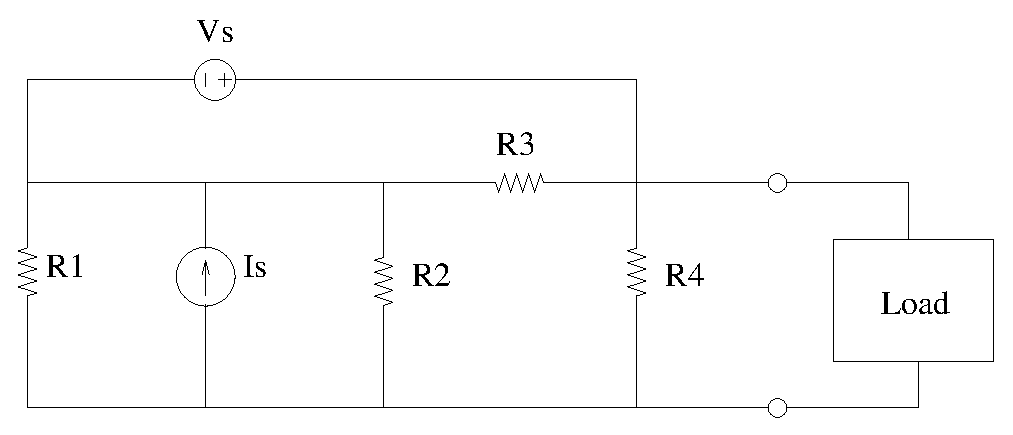
\includegraphics[width=0.7\linewidth]{p3/p3} 
\caption{Big senior project circuit}
\label{fig:p3}
\end{minipage}\hfill
\begin{minipage}[l]{0.25\linewidth}
\begin{tabular}{|l|l|}
\hline
Component & Value \\ \hline
$V_s$ & 5 V \\ \hline
$I_s$ & 1 A \\ \hline
$R_1$ & 5 $\Omega$ \\ \hline
$R_2$ & 10 $\Omega$ \\ \hline
$R_3$ & 10 $\Omega$ \\ \hline
$R_4$ & 20 $\Omega$ \\ \hline
\end{tabular}
\end{minipage}
\end{figure}

Unfortunately the other members of your group dropped the ball and only bought
a single ideal current source.  At first you panic, but then you realize that
you learned some tricks in ECE110L that will save the day.  

\begin{enumerate}
    \item Construct the Norton equivalent circuit for the circuit shown in
        Figure~\ref{fig:p3}.  Clearly solve for, draw and label the Norton
        equivalent circuit.  How much current does the current source need to
        provide, and what value resistor do you need for your circuit?

    \item After building your Norton equivalent circuit, you realize that the
        current source that your group ordered is a dud.  Just as you make this
        realization, a friend walks by the lab and offers you an ideal voltage
        source that you can use for your project.  Clearly solve for, draw and
        label the Th\'{e}venin equivalent circuit for the circuit shown in
        Figure~\ref{fig:p3}.  How much voltage does the voltage source need to
        provide, and what value resistor do you need for your circuit?
\end{enumerate}
